%==============================================================================
% Casus onderzoeksproces: Database-performantie
%==============================================================================
% Gebaseerd op LaTeX-sjabloon ‘Stylish Article’ (zie artikeltin.cls)
% Auteur: Jens Buysse, Bert Van Vreckem

% Compileren document:
% 1) latexmk -pdf db-performance
% 2) biber db-performance
% 3) latexmk -pdf db-performance

\documentclass[fleqn,10pt]{artikeltin}
\usepackage{graphicx} % Required for including pictures
\graphicspath{{figures/}} % Specifies the directory where pictures are stored
%------------------------------------------------------------------------------
% Metadata over het artikel
%------------------------------------------------------------------------------

\JournalInfo{HoGent Bedrijf en Organisatie} % Journal information
\Archive{Onderzoekstechnieken 2016 - 2017} % Additional notes (e.g. copyright, DOI, review/research article)

%---------- Titel & auteur ----------------------------------------------------

\PaperTitle{Performantievergelijking van database-systemen}
\PaperType{Casus onderzoeksproces} % Type document

\Authors{Voornaam Naam\textsuperscript{1}, Voornaam Naam\textsuperscript{2}, Voornaam Naam\textsuperscript{3}, Voornaam Naam\textsuperscript{4}} % Authors
\affiliation{\textbf{Contact:}
  \textsuperscript{1} \href{mailto:voornaam.naam@student.hogent.be}{voornaam.naam@student.hogent.be};
  \textsuperscript{2} \href{mailto:voornaam.naam@student.hogent.be}{voornaam.naam@student.hogent.be};
  \textsuperscript{3} \href{mailto:voornaam.naam@student.hogent.be}{voornaam.naam@student.hogent.be};
  \textsuperscript{4} \href{mailto:voornaam.naam@student.hogent.be}{voornaam.naam@student.hogent.be}}

%---------- Abstract ----------------------------------------------------------

\Abstract{ Hier komt de samenvatting van het artikel, als een doorlopende tekst van één paragraaf. Schrijf dit pas helemaal op het einde, als de inhoud al op punt staat. Volgende elementen moeten hier zeker in vermeld worden: de \textbf{context} (waarom is dit werk belangrijk?), de \textbf{nood} (waarom moet dit onderzocht worden?), de \textbf{taak} (wat is er precies uitgevoerd waarover in dit artikel gerapporteerd wordt?), het \textbf{object} (wat staat in dit document geschreven?), het \textbf{resultaat}, de belangrijkste \textbf{conclusie} en \textbf{perspectief} (welk vervolgonderzoek zou er hierna kunnen uitgevoerd worden?). }

%---------- Onderzoeksdomein en sleutelwoorden --------------------------------

\newcommand{\keywordname}{Sleutelwoorden} % Defines the keywords heading name
\Keywords{Database-beheer. Relationele databases --- performantie} % Keywords

%---------- Titel, inhoud -----------------------------------------------------
\begin{document}

%\flushbottom % Makes all text pages the same height
\maketitle % Print the title and abstract box
\tableofcontents % Print the contents section
\thispagestyle{empty} % Removes page numbering from the first page

%------------------------------------------------------------------------------
% Hoofdtekst
%------------------------------------------------------------------------------

% Er is al een zekere structuur gegeven hieronder, maar pas dit aan als dat zinvol is (bv. uitvoeren experimenten en analyse resultaten in aparte sectie, enz.).

\section{Inleiding} % The \section*{} command stops section numbering
\label{sec:inleiding}

Beschrijf in deze sectie de context (dit houdt ook literatuuroverzicht in), nood en taak. Hier horen veel literatuurverwijzingen thuis, minstens naar~\textcite{Bassil2012}.

Een typische laatste zin voor de inleiding is ``De rest van dit artikel is als volgt gestructureerd: Sectie~\ref{sec:LiteratuurStudie} bevat de Literatuur studie, Sectie~\ref{sec:methodologie} beschrijft de gevolgde methodologie, Sectie [...]''

\section{Literatuur studie}
\label{sec:LiteratuurStudie}
\textbf{Basil 2012}
Om het artikel samen te vaten in een paar zinnen zou ik zeggen dat het gaat over verscheidene DBMS die getest worden op performantie doormiddel van complexe en minder complexe queries. De performantie werd gemeten door het geheugen gebruik, cpu gebruik, thread count en de duurtijd om het uit te voeren. De geteste DBMS zijn MS SQL Server 2008, Orracle 11g, IBM DB2, MySQL 5.5 en MS Access 2010\\

\textbf{Huge and Real-Time Database Systems: A Comparative Study and Review for SQL Server2016, Oracle 12c and MySQL 5.7 for Personal Computer}
Dit artikel gaat ook over het testen van verscheidene DBMS doormiddel van queries. Alleen testen ze niet altijd op dezelfde dataset maar op verschillende groottes van sets. De queries worden niet getoond maar ze schetsen wel kort wat de bedoeling van de query was. Ten opzicht van het artikel van Basil testen ze meer aspecten van een DBMS.\\

\textbf{Comparing nosql mongodb to an sql db}
Dit artikel gaat over het vergelijken van de NoSQL DBMS: MongoDB en de SQL DBMS: SQL Server. Dit doen ze door te testen op de snelheid van insert, update en select operaties. Wat weliswaar enkel op een database van bescheiden formaat wordt uitgevoerd. Ten opzichte van Basil wordt er hier wel op minder aspecten getest.\\

\textbf{MySQL Database Management System Forks Comparison and Usage}
Dit artikel gaat over het vinden van de beste oplossing in de MySQL database management system familie. Voor het vinden van de beste oplossing testen we drie grote MySQL DBMS branches die momenteel aan de top staan: Percona Server, MariaDB en MySQL Community Server. Op deze drie DBMS voeren ze een analyse uit van de storage engines, performance metrics en beschikbare oplossingen voor backup en restore procedures.\\

\textbf{Evalution Of Database Management Systems, Bachelor's Thesis in Computer Engineering, Xing Liang and Yongyu Lu}
In dit artikel worden verschillende DBMS systemen vergeleken. Er wordt eerst een selecties gemaakt adhv verschillende requirements. Deze selectie van systemen worden dan aan verschillende testen onderworpen met behulp van 'simpele' queries. Volgens deze analyse is Firebird de beste DBMS. Dit artikel sluit zeer nauw aan bij onze onderzoeksvraag.\\


Het artikel van Jari (1) bespreekt DBMS op meerdere soorten query’s maar het is wel spijtig dat de query’s zelf niet getoond worden. Ook meer gegevens dan de uitvoertijd zouden een mooie aanvulling geweest zijn. In de bespreking van de experimenten worden er steeds maar een paar DBMS bijgehaald en niet altijd allemaal. In het artikel zijn er ook afbeeldingen maar die geven niet altijd even duidelijk weer wat er precies gebeurt is. Soms staat er enkel een grafiek voor één bepaalde DBMS, maar in de uitleg die bij het experiment staat worden er meerder DMBS aangehaald. En als er in een experiment meerdere worden aangehaald, worden ze er niet allemaal bij betrokken maar enkel een paar. Voor de rapportering van de resultaten zou het beter geweest zijn als ze ten eerste altijd elk DBMS zouden testen op hetzelfde vlak en niet steeds één staaf op de grafiek voor drie DBMS. Ten tweede testen met steeds dezelfde dataset en niet steeds met een andere zou ook een beter algemeen beeld geven van de DBMS. De resultaten zijn niet statistisch significant, want er word niet steeds getest op dezelfde dataset noch met alle DBMS vermeld in de titel. Dit kunnen we afleiden uit het artikel omdat op de afbeeldingen worden er op de x-as steeds een paar DMBS gezet en in de bespreking worden ze ook vermeld.\\

Het artikel van Billy (2) bespreekt MongoDB en SQL Server op meerdere soorten query’s maar het is wel spijtig dat de query’s zelf niet getoond worden. Ook meer gegevens dan de uitvoertijd zouden een mooie aanvulling geweest zijn. In dit artikel wordt er wel goed vergeleken tussen de twee DBMS en de soorten queries. In het artikel zijn er afbeeldingen beschikbaar maar die geven niet altijd een even duidelijk weer hoeveel uitvoeringstijd de query heeft bij een bepaalde test case. De resultaten worden goed weergegeven en vergeleken, alleen mocht de data van de grafieken apart worden meegegeven in een tabel of een aparte excel file. Elke DBMS doorloopt alle queries en per query worden alle test cases getest, hierdoor zijn de resultaten statistisch significant.\\

In het artikel van Robin (3) gaat het over drie DBMS van de MySQL database management system familie die worden vergeleken. Doordat de bekomen informatie van de drie DBMS uit de MySQL database management system familie komen, kunnen de resultaten niet worden vergeleken met andere DBMS. Alle resultaten worden goed weergegeven. Bij elk onderdeel is het duidelijk wat er getest werd en wat erop de grafieken en tabellen staat. Uit de paragraaf waar ze uitleg geven over de test omgeving, kunnen we afleiden dat elke DBMS een identieke configuratie heeft met dezelfde waarden en parameters.\\

In artikel van Frédéric (4) word zeer duidelijk besproken welke DMBS er worden geselecteerd om een focus op te leggen. Ondanks dat de onderzoeksvraag over de algemene performantie van DBMS gaat, gaat het artikel eerder over het beantwoorden van de noden van een applicatie in plaats van de algemene performantie. Desondanks het verschil lopen deze 2 artikelen wel in grote lijnen gelijk.In het artikel worden alle resultaten zeer duidelijk en geordend weergegeven. Er word per criteria een duidelijke beschrijving weergegeven waarom het ene beter of slechter is dan het andere.\\

Het begrip performantie is geen éénduidig begrip, want het kan veel meer inhouden dan alleen snelheid. Het kan ook zijn dat de hoeveelheid gebruikt geheugen belangrijk is of het cpu gebruik. Bijgevolg is performantie niet éénduidig. Voor performantie te testen zouden we met een groot aantal parameters rekening moeten houden. Voor deze analyse hebben we ons beperkt op de belangrijkste parameters. De performantie kunnen we concreet meten door steeds dezelfde query keer op keer testen en alle resultaten bijhouden en opslaan eer je een ander DBMS test met diezelfde query met hetzelfde aantal tests.

\section{Methodologie}
\label{sec:methodologie}

\textbf{Uitvoeren experimenten}

Laptop van Jari: Dell Inspiron 15 
Processor Intel(R) Core(TM) i7-6700HQ CPU @ 2.60GHz, 2601 MHz, 4 core('s), 8 logische processor(s). 
Ram Geïnstalleerd fysiek geheugen (RAM)	16,0 GB

Laptop van Robin: Lenovo ideapad 520
Processor	Intel(R) Core(TM) i7-7500U CPU @ 2.70GHz, 2904 MHz, 2 core('s), 4 logische processor(s)
Geïnstalleerd fysiek geheugen (RAM)	12,0 GB

Laptop van Frédéric: Asus UX510UXK
Intel(R) Core(TM) i7-7500U CPU @ 2.70GHz, 2904 MHz, 2 core('s), 4 logische processor(s)
Geïnstalleerd fysiek geheugen (RAM)	8,0 GB

\title{Opstart VM}

1. Downloaden van repository taak (niet clonen want dit geeft problemen met de conversie van EOF van Windows die github automatisch doet).
2. Navigeren naar de map "experiment" (via git bash)
3. Door het commando "vagrant up" word de VM aangemaakt.
4. Als hij klaar is geeft u het commando "vagrant ssh".
5. Het script dat wij gemaakt hebben vereist een installatie van "time", dit moet als user root dus voert u het commando "su -" uit en het wachtwoord is "vagrant".
6. Omdat het beter is de query meermaals te doen uitvoeren hebben we in het script voor elke query onderstaande code geschreven, het voert elke query 50 maal uit.

\#rm ResultQuery1.csv
echo "sys,real,user" >> ResultQuery1.csv
for j in {0..49}
do
{ /usr/bin/time -f "%s,%e,%U" mysql -udbo -pdbo dbo < /vagrant/queries/postgre/query1.sql > /dev/null; } 2>> ResultQuery1.csv;
done 

7. Om "time" te installeren voert u (als root) het commando \framebox[1.1\width]{yum install time}\par uit en geeft u "y" in tot het installeert.
8 Als het klaar is mag u terug naar vagrant user gaan doormiddel van het commando \framebox[1.1\width]{logout}\par . 
9. Om het script uit te voeren moet u het in dezelfde map zetten als de vagrantfile.
10. Om het script te kunnen uitvoeren moet u eerst \framebox[1.1\width]{cd /vagrant}\par uitvoeren zodat u in de juiste map bent.
11. Daar voert u het commando \framebox[1.1\width]{bash script.sh}\par uit en wacht u tot het klaar is.
12. Ons script exporteert .csv bestanden, deze komen in dezelfde map terecht als de vagrant file.

\title{Rstudio berekeningen}

Omdat ons script .csv bestanden exporteert gebruiken we volgend commando om het in te lezen in RStudio.

ResultQuery1 <- read.csv("~/Ho Gent/jaar 2/vakken/semester 2/Onderzoekstechnieken/opdracht/github opdracht/onderzoekstechnieken-casus-master/experiment/ResultQuery1.csv")

Als u niet exact weet welk pad u nodig heeft kan u ook via import dataset (From text (base)) -> navigeren naar bestand -> openen
Dan gaat RStudio in de console het volledige commando tonen dat het gebruikt heeft voor het bestand te importeren en dat gebruikt u dan om de andere bestanden in te laden door de naam aan te passen van de variabele (in het bovenstaande voorbeeld ResultQuery1) en het bestand achteraan.

Om het dataframe vervolgens te bekijken gebruiken we het commando \framebox[1.1\width]{ View(ResultQuery1)}\par.
We willen ook de standaardvariatie dus daarvoor gebruiken we het commando \framebox[1.1\width]{var(ResultQuery1)}\par.
Omdat we ook de boxplot ervan willen gebruiken we het commando \framebox[1.1\width]{summary(ResultQuery1)}\par.
Als laatste willen we ook de standaard afwijking, maar onze csv heeft drie kolommen dus willen we eerst de kolom met effectieve tijden eruit halen. Daarvoor geven we het commando \framebox[1.1\width]{x <- ResultQuery1[,"real"]}\par. Daarin is de "x" de variabele, ResultQuery1 de dataframe en "real" is de kolom die we willen.
Om vervolgens de standaard afwijking te laten berekenen geven we \framebox[1.1\width]{sd(x)}\par in.

\title{Postgre installeren}

Om postgre te installeren, voert u als root user (su -) dit commando uit :
 
  \framebox[1.1\width]{yum install https://download.postgresql.org/pub/repos/yum/10/redhat/rhel-7-x86\_64/pgdg-centos10-10-2.noarch.rpm} \par

Vervolgens voert u
  \framebox[1.1\width]{yum install postgresql10}\par
  \framebox[1.1\width]{yum install postgresql10-server}\par
  \framebox[1.1\width]{/usr/pgsql-10/bin/postgresql-10-setup initdb}\par
uit

Daarna moet u het proces bij uw opstart processen zetten door :

 \framebox[1.1\width]{systemctl enable postgresql-10}\par 

Om de service dan te starten
 \framebox[1.1\width]{ systemctl start postgresql-10}\par

Dan moet u een nieuw paswoord instellen 
  \framebox[1.1\width]{sudo -u postgres psql postgres}\par
 
Dan staat er normaal postgres-\# als command prompt (links onderaan)
Daarna voert u \\password postgres uit om een wachtwoord in te stellen (in mariadb was dit 'dbo')
Dan sluit u postgres af door \\q uit te voeren

Om dan ervoor te zorgen dat de databank werkt op redhat moet u navigeren als root user naar de 
/var/lib/pgsql/10/data/ directory.
Daar voert u 
  \framebox[1.1\width]{vi pg\_hba\_conf}\par
  
uit en gaat u doormiddel van het insert status ( 'i' typen) naar onder en past u de lijnen aan van 
  \framebox[1.1\width]{ local all postgres peer}\par
naar 
  \framebox[1.1\width]{ local all postgres md5}\par
 
U kan in plaats van md5 naar trust veranderen als u niet steeds opnieuw het wachtwoord wil ingeven,
dit is echter niet veilig.

Daarna moet u de service herstarten om de file te overschrijven die in gebruik is door 
  \framebox[1.1\width]{sudo service postgresql-10 restart}\par

Dan logt u zicht in als user van postgres
  \framebox[1.1\width]{ sudo su - postgres}\par
en daarna opent u het postgreSQL command promt 
 \framebox[1.1\width]{psql}\par

U moet een user aanmaken
  \framebox[1.1\width]{CREATE USER dbo WITH PASSWORD 'dbo';}\par

Maak dan een databank aan, hier is dbo de naam maar dit mag u uiteraard anders noemen
 \framebox[1.1\width]{ CREATE DATABASE dbo}\par

Daarna moet u het script uitvoeren dat de tabellen aanmaakt maar daarvoor moet u eerst nog het dateformaat 
aanpassen door 
 \framebox[1.1\width]{'sed -i 's/0:00*/:/g' cd /vagrant/data/invoice.csv }\par

Dan moet u navigeren naar waar de file staat die de tabellen aanmaakt.
Daar voert u het script uit met 
 \framebox[1.1\width]{ psql -U dbo -f create\_tables.sql (dit moet in de gewone vagrant command prompt(links onderaan))}\par

Dan maakt u een script aan om de csv bestanden in te laden
 \framebox[1.1\width]{\#!/bin/bash
  	\# load csv files into postgreSQL database

	function load\_csv {
			local csv\_path=\$1
			local file="\${csv\_path\#\#*/}"
			local table\_name="\${file\%\%.*}"

			sudo psql -U dbo -d dbo -c "\\copy \${table\_name} FROM '\${csv\_path}' DELIMITER ';' CSV HEADER;";
	}

	dir=/vagrant/data

	for file in "\${dir}"/*.csv; do
			load\_csv "\${file}"
	done}\par
In de .sql bestanden met de queries verwijdert u overal de 'dbo.' bijvoorbeeld bij query10.sql past u dus in de WHERE clause "dbo.invoicedetail" aan naar "invoicedetail"
Daarna moet u de queries door een conversietool halen voor de andere syntax die postgre heeft. 
Wij hebben http://www.sqlines.com/online gebruikt. Daar selecteert u links mysql en rechts postgresql

Omdat de syntax van Postgre iets anders is om een query uit te voeren hebben we van bovenstaande script van mariadb een kleine aanpassing gemaakt, we hebben per query dit gemaakt:
\#rm ResultQuery1.csv
echo "sys,real,user" >> ResultQuery1.csv
for j in {0..49}
do
{ /usr/bin/time -f "\%s,\%e,\%U" psql -U dbo -f query1.sql > /dev/null; } 2>> ResultQuery1.csv;
done 

\section{Experimenten}
\label{sec:experimenten}

Beschrijf hier hoe de experimenten verlopen zijn en de belangrijkste resultaten. Voeg ook tabel(len) en figuren toe.

\begin{figure}
    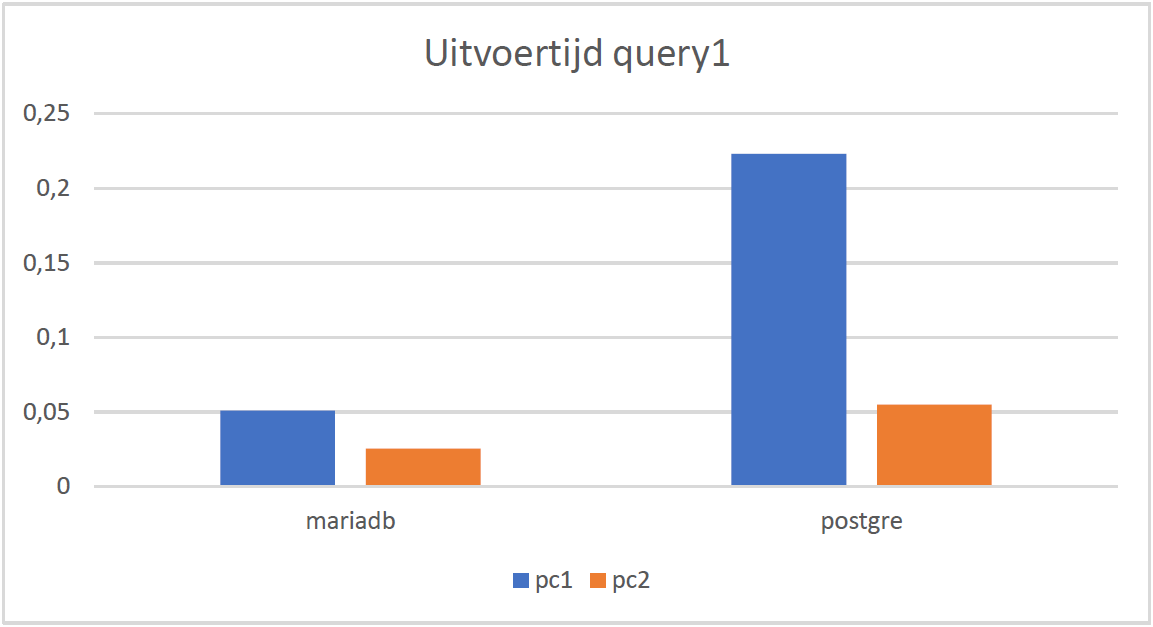
\includegraphics[width=0.5\textwidth]{query1.png}
\end{figure}

Beschrijf zeker ook de uitkomst van de statistische toets: zijn de verschillen in performantie significant?

\section{Conclusie}
\label{sec:conclusie}

Beschrijf hier de conclusie en eventuele bijkomende onderzoeksvragen die in een verder onderzoek kunnen uitgediept worden

%------------------------------------------------------------------------------
% Referentielijst
%------------------------------------------------------------------------------

\phantomsection
\printbibliography[heading=bibintoc]

\end{document}
